\chapter{\chapviiname}
\label{chapter7}



\begin{abstract}
	\lipsum
\end{abstract}



\section{INTRODUCTION} % 1.5 pages
\label{sec:introduction}
% Breifly discuss: the state of the art of DEGs, previous device created, and the intention of this chapter: To elucidate the operation of the DEA-EIT device specifically looking into it's potential function as a DEG.
A DEAs and Dielectric Elastomer Generators (DEGs) share a similar form whereby they both have compliant conductive electrodes either side of a dielectric elastomer (DE) membrane. However, DEGs represent a class of electromechanical devices that harness mechanical strain to generate electrical energy. DEAs and DEGs can often utilised the same soft electroactive area for actuation and power generation, but differ in the connected electronics. These devices exploit the properties of dielectric elastomers, which are soft, flexible materials capable of undergoing significant deformation. This deformation can be utilised to generate electrical power, making DEGs a promising technology for energy harvesting applications and also an unintended consequence of loading a DEA device.

In typical DEG configurations, the focus has been on uniform, global strain changes within the dielectric elastomer domain. Previous research has concentrated on scenarios where the entire thickness of the DE is reduced as a result of applied strain, leading to energy generation due to global DE deformations \cite{Carpi2015, Savage2012, Koh2009}.

In contrast, this work explores unintentional DEG scenarios that have arisen from the invention of a hybrid actuation and pressure mapping DEA-EIT device. By investigating the effects of localised thickness reduction within the DE caused during a pressure mapping load event during DEA switching we observe unintended power generation due to the change in the device capacitance. This localised approach introduces a new dimension to DEG functionality, where strain is not uniformly applied but concentrated in specific areas. This integration allows for precise monitoring and analysis of localised deformations, thereby enhancing the understanding and potential applications of DEGs in advanced energy harvesting and sensing technologies. In the existing literature, neither the intentional nor unintentional use of a DEA-EIT device as a DEG, when subjected to localised loads, has been investigated as of the time of writing this work.



\subsection{BACKGROUND} 
\label{subsec:background}
% Re-iterate in a few sentences how the DEA-EIT sytstem works
Before describing how a dielectric generator arises in DEA-EIT device, it is important to understand the function of a DEA-EIT device first as  described in detail in the previous chapter. A DEA-EIT device can use the same compliant electrodes and dielectric elastomer to function both as an electro-active actuator and pressure mapping sensor. The DEA function consists of applying a high voltage to a bottom electrode leaving the top electrode as the low voltage electrode which performs as the pressure mapping surface. The pressure mapping surface is piezoresistive and uses electrical impedance tomography to map any changes in resistance and hence any loads throughout the electrode surface. 
\begin{figure}[H]
	\centering
	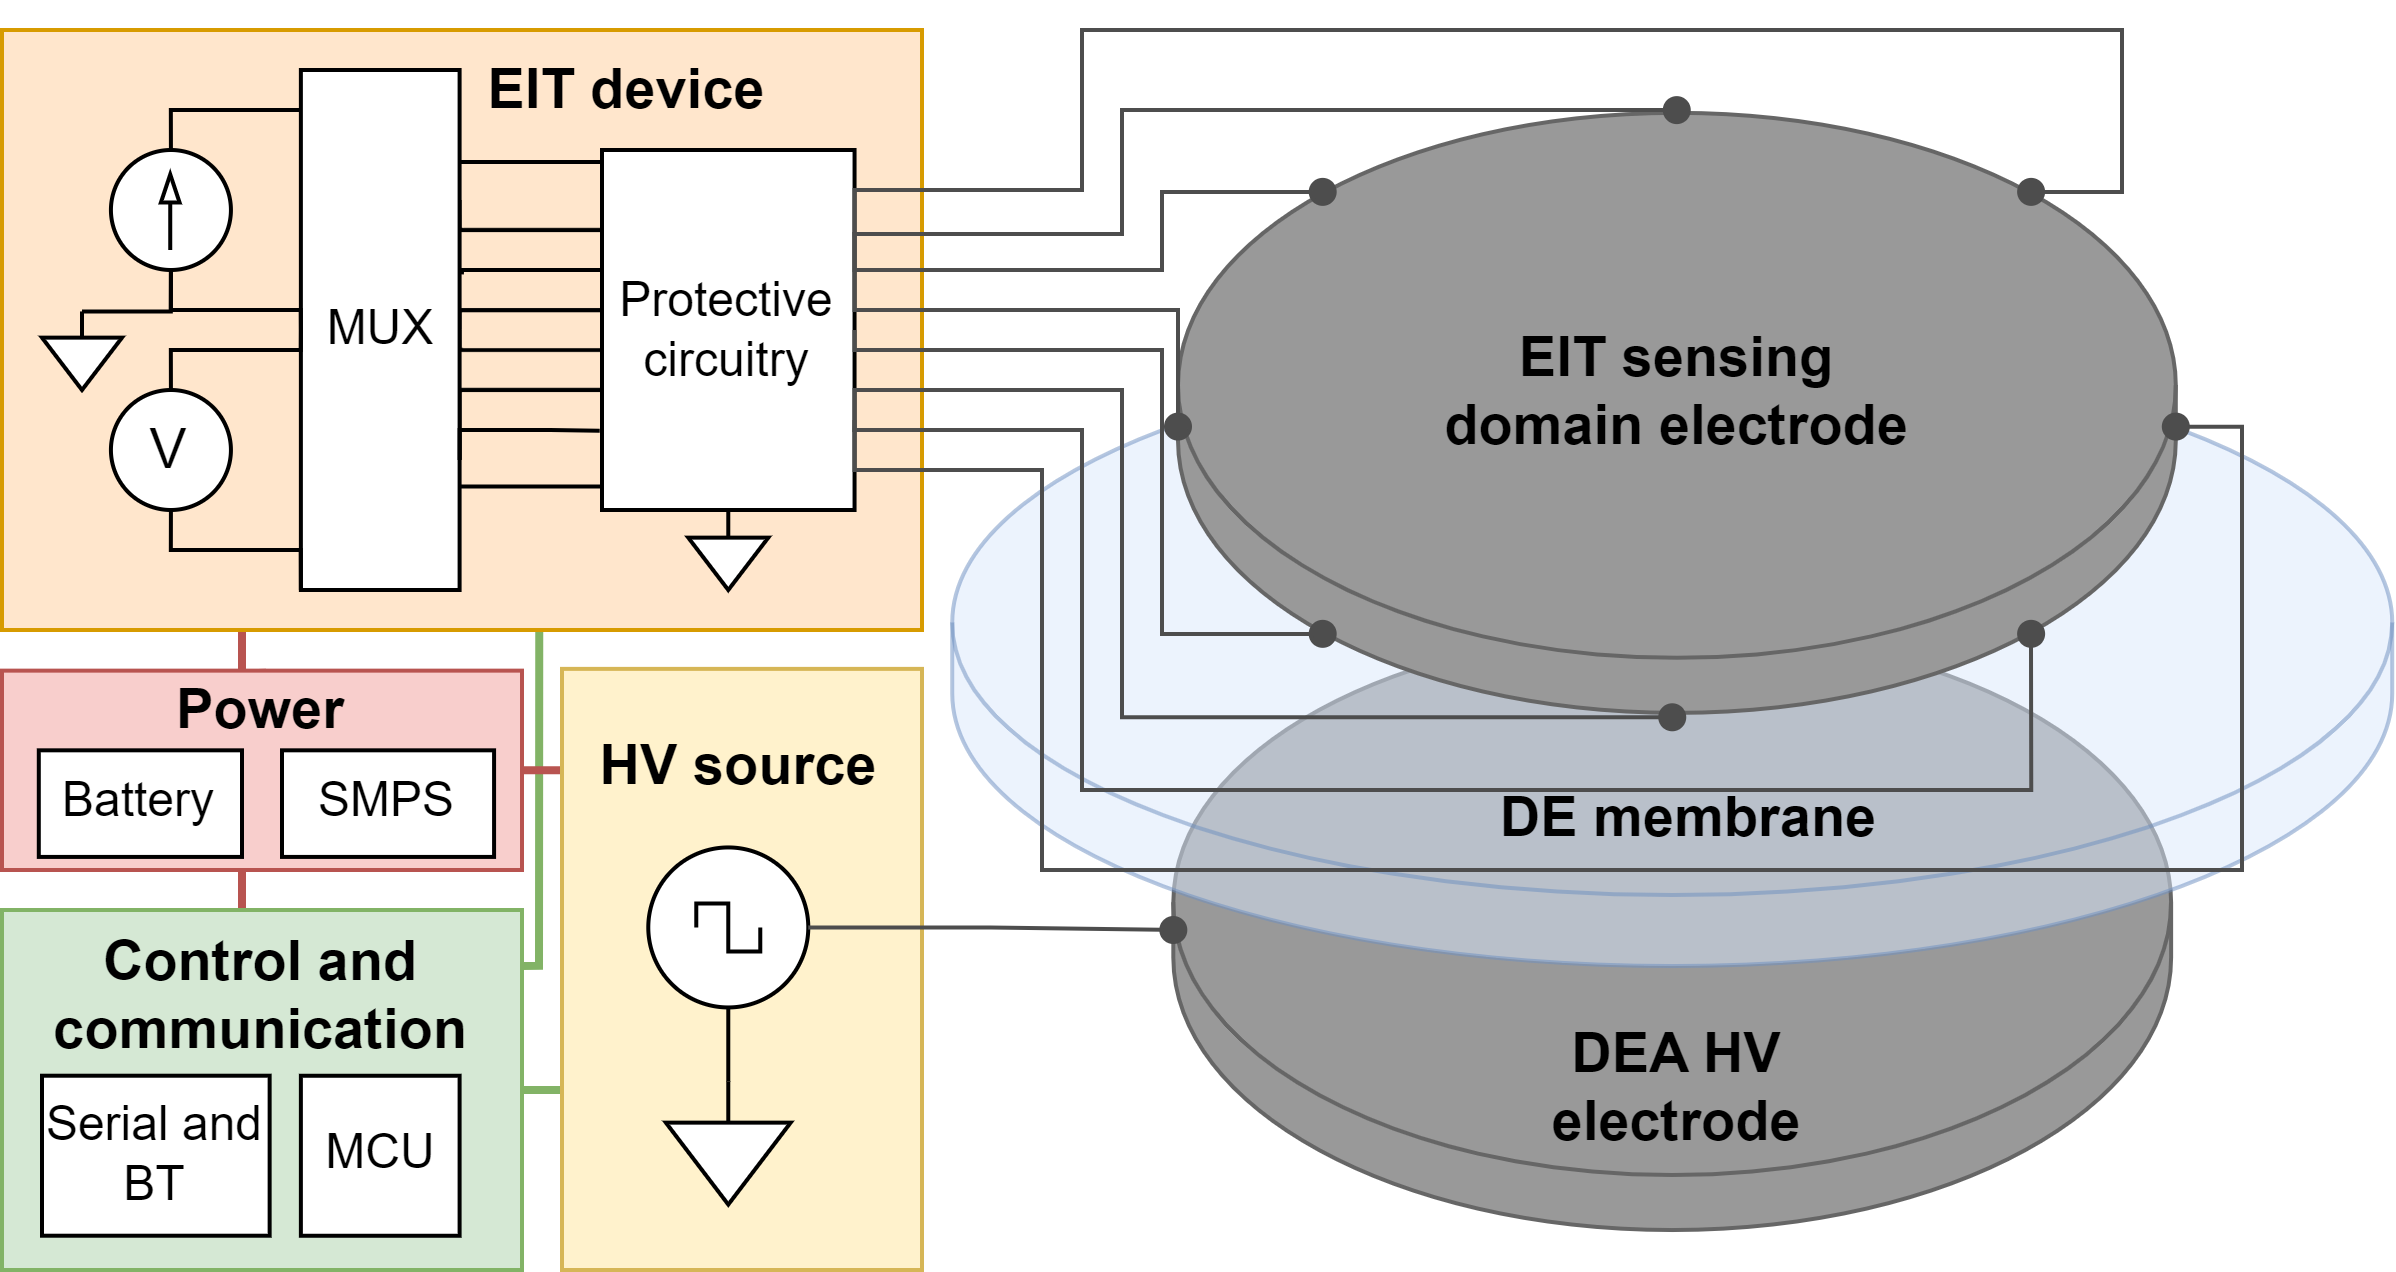
\includegraphics[width=0.8\linewidth]{Figures/DEA-EIT_architecture.png}
	\vspace{0.3cm}
	\caption{Architecture of a DEA-EIT pressure mapping and actuator device.}
	\label{fig:dea-eit-architecture-w-MCU}
\end{figure}

A DEG may be incidentally be created during simultaneous DEA-EIT operation. This effect will take place when the DEA experiences sufficiently large external strains and DEA voltage switching at specific times.

\begin{figure}[H]
	\centering
	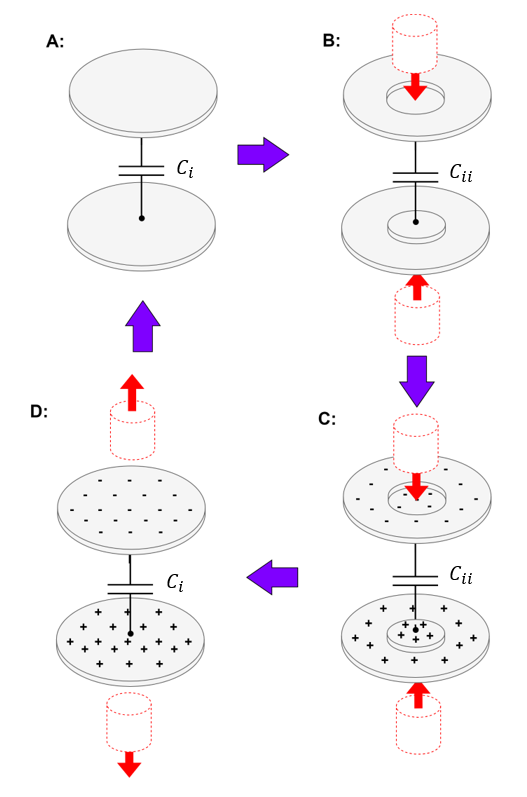
\includegraphics[width = 0.5\textwidth]{Figures/DEA-EIT_DEG_ckt_simple.png}
	\vspace{0.2cm}
	\caption{Dielectric elastomer generator scenario with a localised compressive load}
	\label{fig:dea_eit_deg}
\end{figure}
Where $C_i$ is the initial capacitance of the DEA, $C_{ii}$ is the `primed' capacitance of the DEA, the positive and negative signs, $+$ and $-$, on the compliant electrode represent electrical charge, and the red cylinder represents the load applicator. The typical operation of a DEG consists of the five main stages described below and exemplified in Figure \ref{fig:dea_eit_deg}.
% Fill with wonderful electrostatics/electrical equations

\textbf{State A}: the DEA has an initial capacitance of $C_i$ and is deformation free and has zero voltage applied across the compliant electrodes.

\textbf{State B}: the DEA is compressed deformed with a localised change(s) in thickness of the DE, $\Delta z$, increasing the DEA capacitance to $C_{ii}$. Work is done on the DEA by the compressive load storing elastic potential energy in the strained DE and the compliant electrodes.
As derived from Hooke's law the elastic potential energy, $U_{\varepsilon}$ for a material of Young's modulus, $Y$, cross-sectional area, $A_i$, original thickness, $z_i$, and change in thickness, $\Delta z$ is given in Equation \ref{eqn:elastic-energy}. This equation is for a singular body showing the core parameters governing the elastic potential energy.
% Todo: mention that this equation isn't suffice so we use FEM modelling which gives a better representation of the Hookean continuum model but still neglects viscous damping within the material.
\begin{equation}
	U_{\varepsilon} = \frac{YA_0\Delta z^2}{2z_i}
	\label{eqn:elastic-energy}
\end{equation}

\textbf{State C}: the DEA electrodes are charged with an applied voltage across the compliant electrodes, $V_i$. The total charge developed is $Q$ as given by Equation \ref{eqn:charge-cap-volt1}.
\begin{equation}
	Q = C_{ii}V_{i}
	\label{eqn:charge-cap-volt1}
\end{equation}
Charging the electrodes gives electrical potential energy to the DEA as it is now a charged capacitor. The electrical potential energy of the DEA is given by Equation \ref{eqn:elec-energy1}.
\begin{equation}
	U_{EC} = \frac{1}{2}C_{ii}V_i^2
	\label{eqn:elec-energy1}
\end{equation}

\textbf{State D}: The DEA is unloaded and returns to its original state with capacitance, $C_i$, while maintaining the same charge $Q$ causing the voltage to increase to $V_{ii}$ as shown by Equation \ref{eqn:charge-cap-volt2}.
\begin{equation}
	V_{ii} = \frac{Q}{C_{i}}
	\label{eqn:charge-cap-volt2}
\end{equation}
When the load is released the elastic potential energy, $U_{\varepsilon}$, is used as the DEA returns to a relaxed state. In parallel, the increase in voltage on the DEA increases the electrical potential energy, $U_{ED}$ as shown by Equation \ref{eqn:elec-energy2}.
\begin{equation}
	U_{ED} = \frac{1}{2}C_{i}V_ii^2
	\label{eqn:elec-energy2}
\end{equation}
Resulting in a gain of electrical potential energy $\Delta U_E$ comprising the difference of $U_{EC}$ and $U_{ED}$.

\textbf{State A*}: The DEA is discharged into the energy harvesting circuit returning the charge and voltage values across the DEA to zero, returning to State A. 
The unintended power generation discussed in the above section may cause issues with the pressure measurement system if switching significantly high DEA voltage source is done during a significant DEA-EIT surface loading event. A significant loading event is one which changes the capacitance of the DEA such that a voltage is generated by the unintended DEG which is high enough to cause potential harm to the EIT driving circuitry. 

An example scenario the extra voltage generated is given. Given that the values from Figure \ref{fig:dea_eit_deg} are, $C_i = 10 pF$, $C_{ii} = 15 pF$, and $V_i = 5 kV$. We get a charge $Q = 75 nC$, and then at stage D, $V_ii = \frac{Q}{C_{i}} = 7.5 kV$. This gives a voltage change, $\Delta V = +2.5 kV$. This voltage change transient is connected to the EIT multiplexer through the capacitance of the DEA.
The multiplexer pins used in this case are limited to between the power rails, i.e. $\pm$22 V \cite{VishayPG2018}. A specified multiplexer further testing would need to be completed on such multiplexer inputs to determine the device's tolerance against transient voltage spikes, as CMOS latch-up may occur \cite{Redmond2001} . 
However, in this case due to the change in capacitance of the DEA the energy generated is $93.75 uJ$ which is less likely to cause damage to the electronic devices.



\section{METHODOLOGY} % 3 pages
\label{sec:method}
% How was the FEM set up? and why?
To confirm the existence of this DEG phenomena in the DEA-EIT device has undergone a sequence of FEM studies. To determine which compressive loads may give significant capacitance changes that could lead to significant voltage amplification and potentially significant energy generation across DEA electrodes, FEA of a DEA undergoing compressive pressure loading events have been completed. Experimental cases using two different loading areas with a range of forces have been completed. The two different loading area given in Figure \ref{fig:FEM_DEA-EIT_loading}. 
\begin{figure}[H]
	\centering
	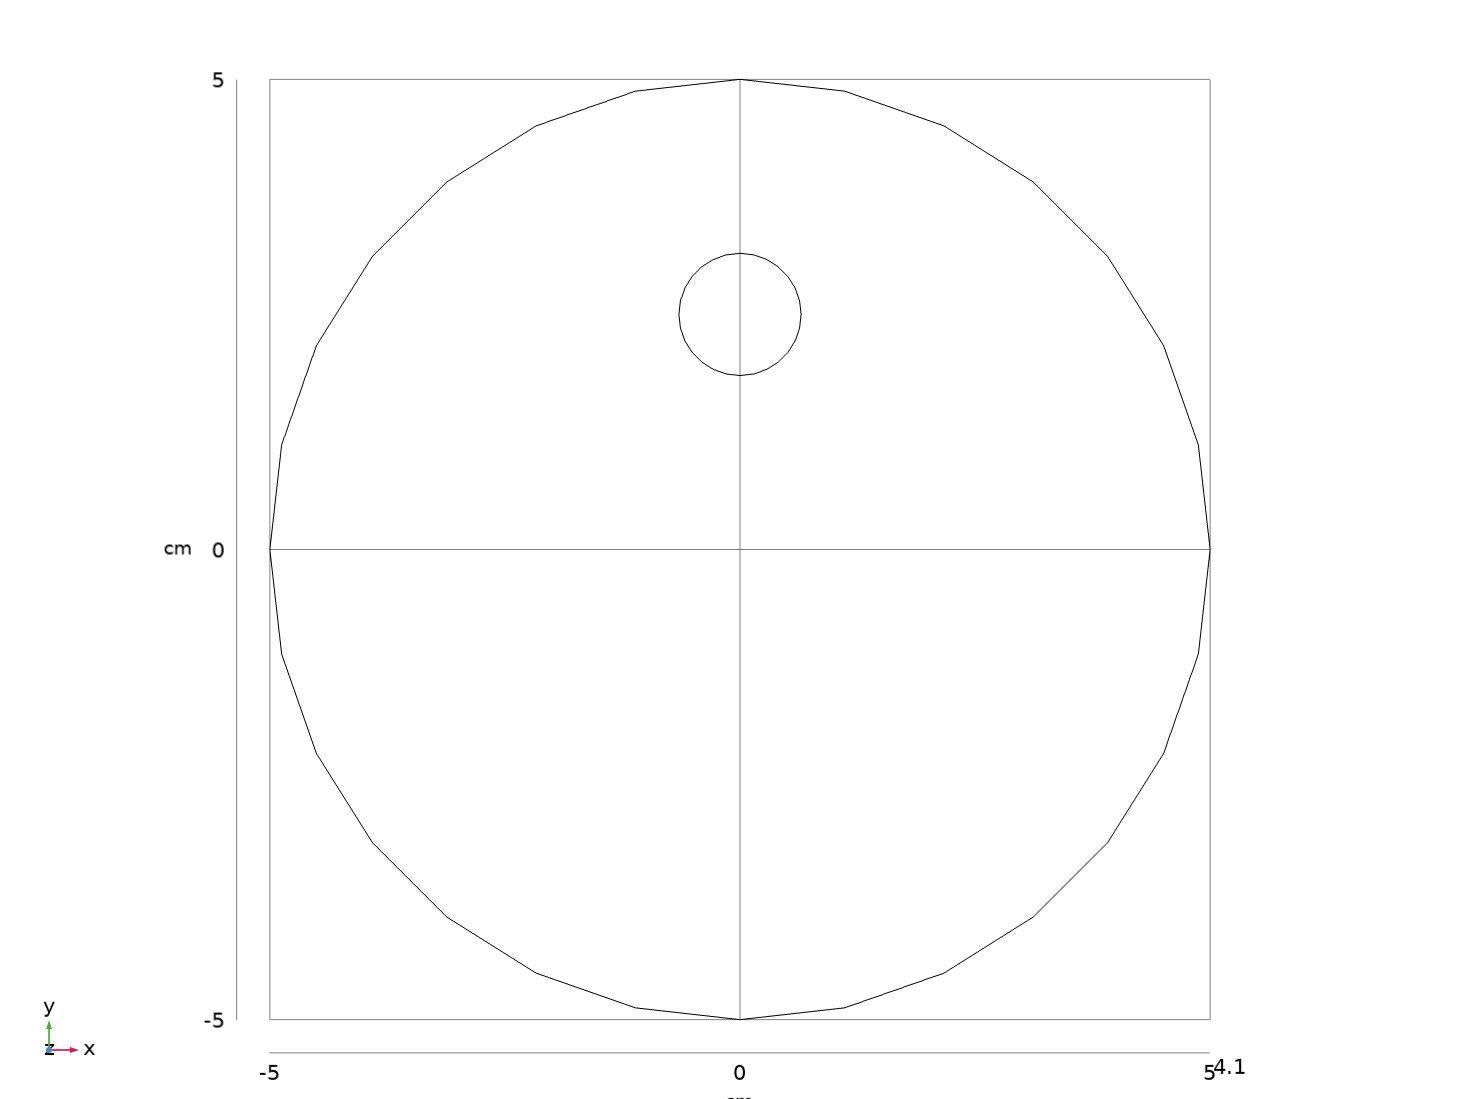
\includegraphics[width=0.45\linewidth]{Figures/d13mm_load_case_comsol2d.png}
	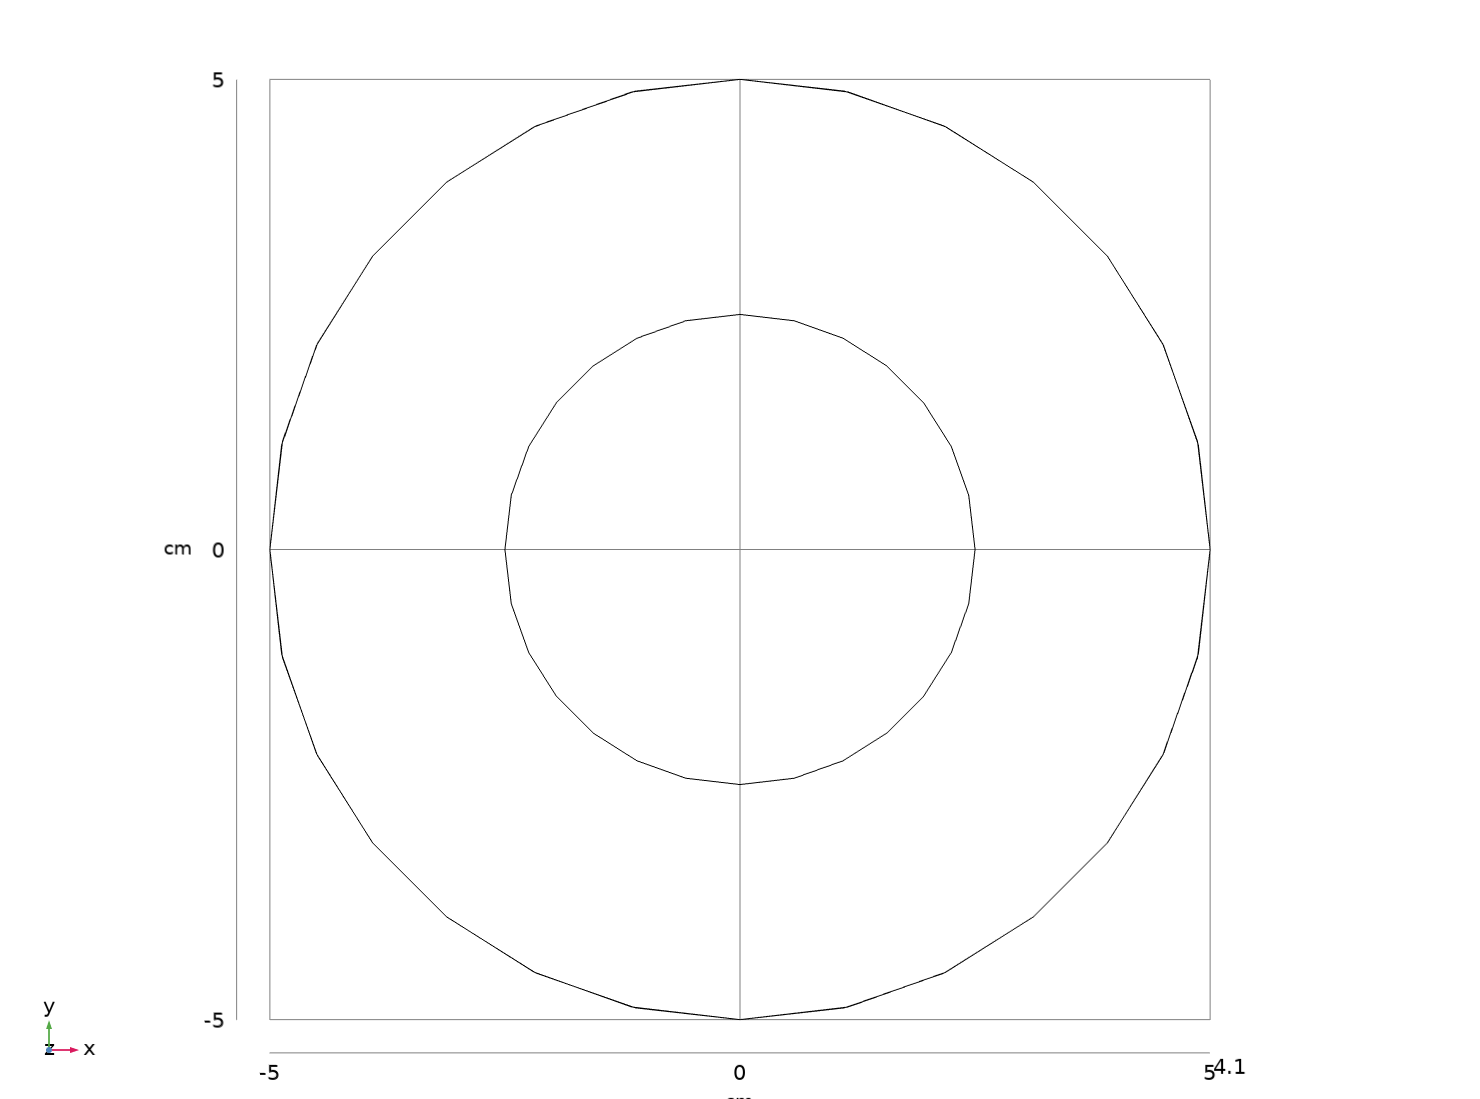
\includegraphics[width=0.45\linewidth]{Figures/d50mm_load_case_comsol2d.png}
	% \includegraphics[width=0.3\linewidth]{multi area touch.png}
	\caption{Loading cases for analysis of capacitance change. Left: 13 mm diameter load. Right: 50 mm diameter load.}
	\label{fig:DEA-EIT_loading}
\end{figure}


\subsection{DEA Load Study}
%% Todo: Describe FEM parameters for DEA loading and FEM tool used!
To obtain a representation of how the DEA structure will deform during a different loading events finite element modelling (FEM) was used to determine the expected deformation of the DEA and create mesh models to use for further electrostatic FEM studies.

The materials used for the FEM load study were closely matched to the characteristics of the material used in previous work \cite{Ellingham2024}. For the compliant electrode a Young's modulus of 100 kPa was used with a Possion's ratio, $\nu_{ce}$ of 0.4, an electrode thickness, $z_{CE}$, of 0.5 mm, and the diameter of 100 mm. The DE material Young's modulus was set to 90kPa with a Poisson's ratio, $\nu_{DE}$, of 0.49, a membrane thickness, $z_{DE}$, of 0.5 mm, and the diameter of 100 mm. 

A static load analysis of the circular areas shown in Figure \ref{fig:DEA-EIT_loading}, for a range of force values. The loads ranged from 2.5 to 240 N, to obtain comparable strain values to those seen within our previous research \cite{Ellingham2021,Ellingham2024} . The bottom electrode surface was assumed fixed in place and rigid to simulate a typical application case where the compliant DEA-EIT material is adhered to a rigid body.

A mesh of the deformed DEA models from each of different load case was saved for use in the next study.


\subsection{Deformed DEA Electrostatics Study}
%% Todo: Describe FEM parameters for DEA capacitance and FEM tool used!
The deformed meshes from the previous load study were used to generate new meshes for an electrostatics study. To determine the change in capacitance from the undeformed DEA model and the deformed DEA cases, an electrostatic study was performed. The same dimensions as the load study were used the compliant electrode was assumed to have an ideal conductivity and the DE membrane relative dielectric permittivity was set to 4.2, the upper limit seen in silicone elastomers. The a positive voltage was set on the upper electrode and the lower electrode was grounded. After the electric field model was generated using COMSOL Multiphysics \cite{COMSOL2022} for each case the compliant electrode capacitance was calculated using Maxwell's capacitance matrices \cite{Smolic2021} . 

\subsection{Voltage and Energy Generation}
The voltage increase and energy generated for each DEA load case was calculated from the capacitance values determined in the electrostatics studies. Analysis of which types of loads can be handled by the DEA-EIT device when undergoing high voltage switching is a critical step for determining the limitations of future applications of the DEA-EIT device.



\section{RESULTS}
\label{sec:results}
The a series of models were generated from a sequence of FEM studies to obtain the voltage and energy generated from a DEA acting as a DEG.

\subsection{Deformed DEA Electrostatics Study}
%% Todo: FEM load plot example (redo!! maybe use the deformed meshes generated?)
%% Todo: Re-run in COMSOL? or re-run with three layers?
\begin{figure}[H]
	\centering
	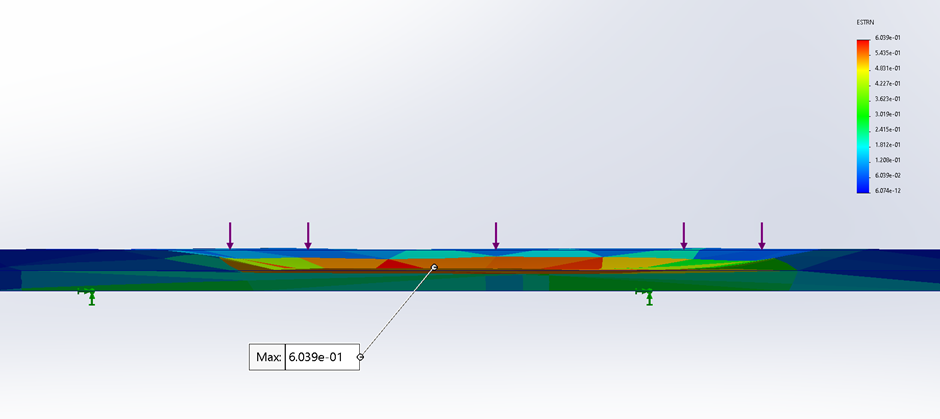
\includegraphics[width=0.6\linewidth]{Figures/d13mm_20N_load_ESTRN_max_FEM.png}
	\includegraphics[width=0.35\linewidth]{Figures/d13mm_20N_load_ESTRN_max_FEM_3d.png}
	\caption{Strain mesh of 13 mm diameter 20 N load case FEM model. Left: Cross-section. Right: 3D view.}
	\label{fig:FEM_DEA-EIT_loading}
\end{figure}


\subsection{Deformed DEA Electrostatics Study}
%% Todo: FEM electric field plot example (redo!!)
%% Todo: re-run with a higher voltage or having a logarithmic scale for electric field lines
\begin{figure}[H]
	\centering
	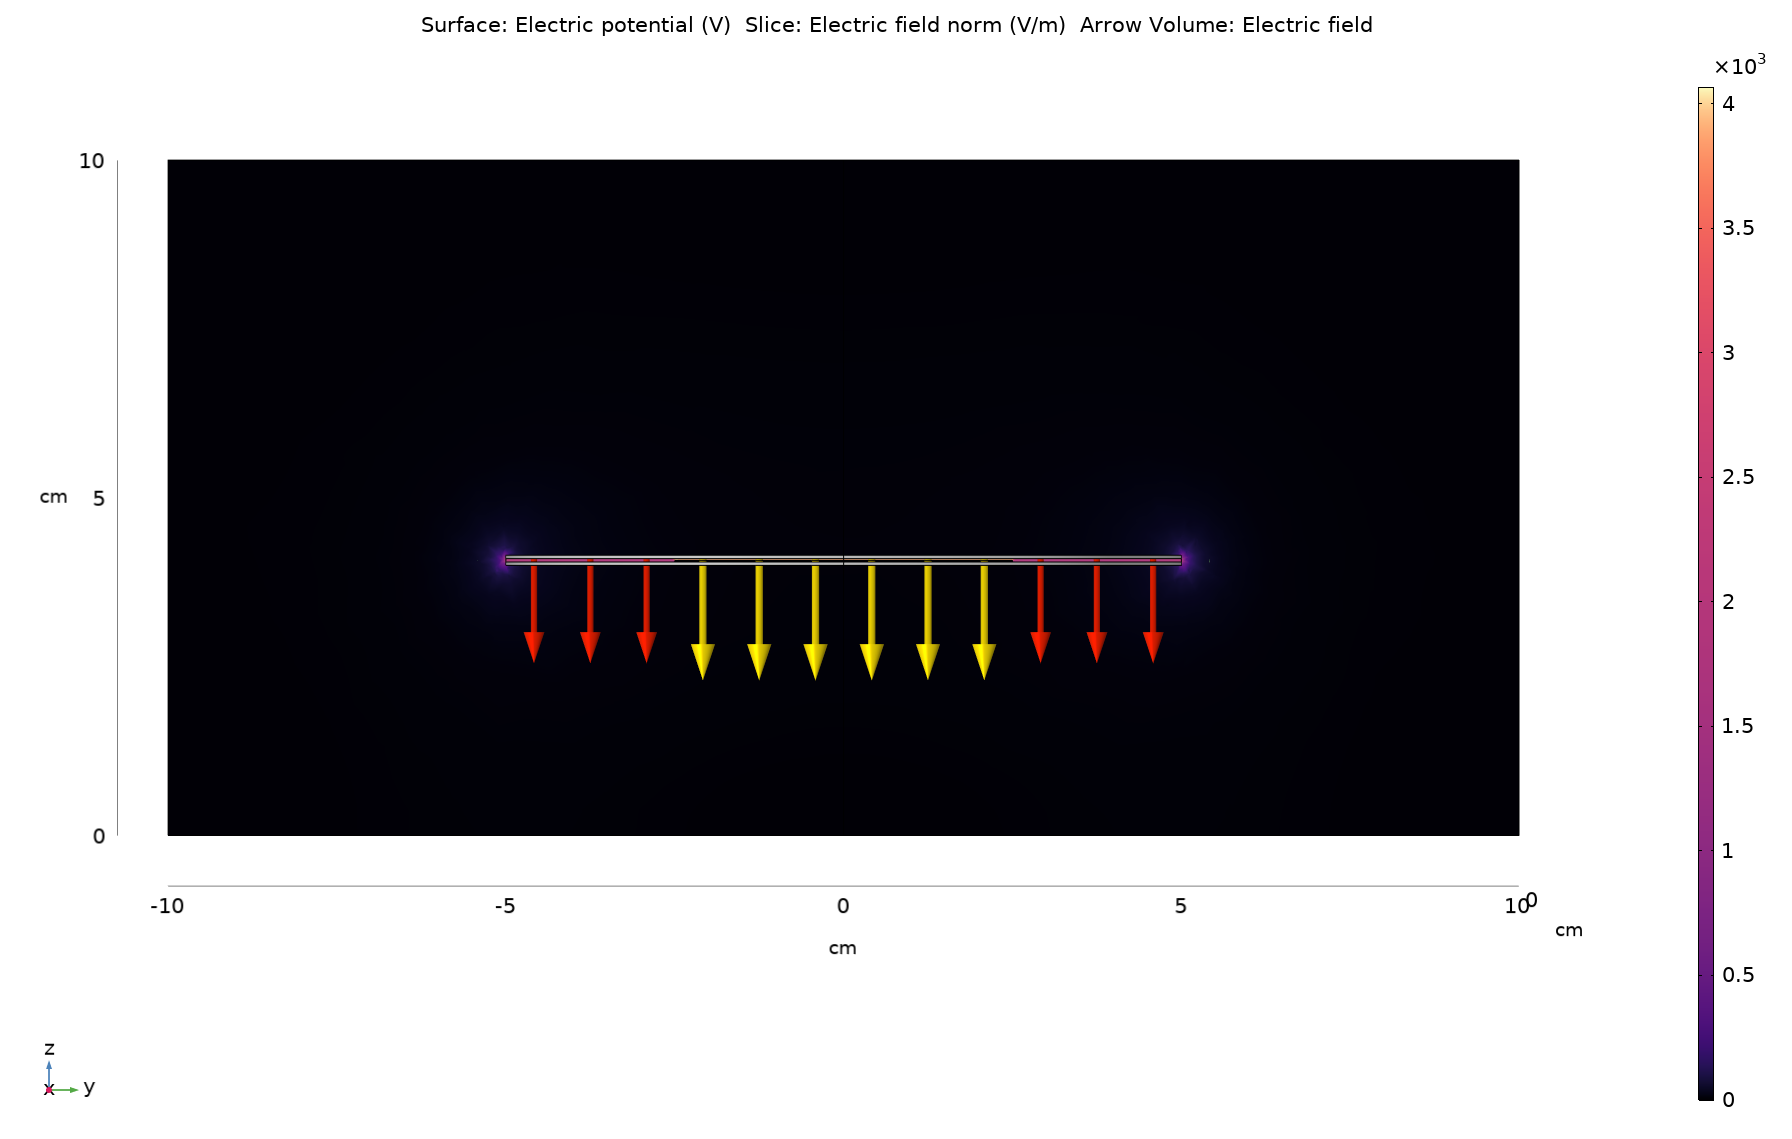
\includegraphics[width=0.6\linewidth]{Figures/d50mm_load_240N.png}
	\includegraphics[width=0.35\linewidth]{Figures/d50mm_load_240N_3d.png}
	\caption{Electric field simulation of 50 mm diameter 240 N load case. Left: Cross-section. Right: 3D view.}
	\label{fig:FEM_DEA-EIT_cap}
\end{figure}


\subsection{Voltage and Energy Generation}
%% Todo: Add energy generated column for each case
\begin{table}[H]
	\centering
	\label{tab:volt-energy-gen-d13mm}
	\caption{Voltage and energy generation results calculated from FEM values for the 13 mm diameter load cases.}
	\vspace{0.3cm}
	\begin{tabular}{llllll}
		\textbf{Load {[}N{]}} & \textbf{ESTRN} & \textbf{C {[}pF{]}} & \textbf{dC {[}pF{]}} & \textbf{dV\_DE {[}V{]}} & \textbf{dU {[}uJ{]}} \\ \hline
		0.00  & 0.00 & 588.86 & 0.00  & 0.00   & 0.00    \\
		2.50  & 0.08 & 589.69 & 0.83  & 7.04   & 31.14   \\
		5.00  & 0.15 & 590.73 & 1.87  & 15.83  & 70.20   \\
		10.00 & 0.30 & 593.40 & 4.54  & 38.25  & 170.68  \\
		20.00 & 0.60 & 605.53 & 16.67 & 137.65 & 630.86  \\
		30.00 & 0.91 & 688.18 & 99.32 & 721.61 & 3903.68
	\end{tabular}
\end{table}


%% Todo: Add energy generated column for each case
\begin{table}[H]
	\centering
	\label{tab:volt-energy-gen-150m}
	\caption{Voltage and energy generation results calculated from FEM values for the 50 mm diameter load cases.}
	\vspace{0.3cm}
	\begin{tabular}{llllll}
		\textbf{Load {[}N{]}} & \textbf{ESTRN} & \textbf{C {[}pF{]}} & \textbf{dC {[}pF{]}} & \textbf{dV\_DE {[}V{]}} & \textbf{dU {[}uJ{]}} \\ \hline
		0.00 & 0.00 & 588.86 & 0.00 & 0.00 & 0.00 \\
		5.00 & 0.01 & mesh   error - too fine & \#VALUE! & \#VALUE! & \#VALUE! \\
		10.00 & 0.02 & 591.90 & 3.04 & 25.68 & 0.20 \\
		20.00 & 0.04 & 595.00 & 6.14 & 51.60 & 0.79 \\
		30.00 & 0.06 & 598.33 & 9.47 & 79.14 & 1.87 \\
		60.00 & 0.12 & 609.24 & 20.38 & 167.26 & 8.52 \\
		120.00 & 0.24 & 635.86 & 47.00 & 369.58 & 43.43 \\
		240.00 & 0.48 & 727.10 & 138.24 & 950.63 & 328.54
	\end{tabular}
\end{table}


\section{DISCUSSION}
\label{sec:concs_disc}
% useful applications
% how to harness it

% harmful use cases
% how to avoid it
Such a voltage generation case may be avoided in an automated system by detecting that a pressure event has occurred and preventing the excitation of the DEA or limiting the charge accumulation on each plate of the capacitor.

% Address idealness of FEM study completed and how physical experimentation could help create a relationship between the simulated and real data in future.

% Overall conclusion ... Can be prevented, only significant if delta C is large, requires more testing, could create a DEG-EIT device to capture data from cars, foot traffic?
